\documentclass{C://Aliases//Dropbox-MIT//Latex_Templates//personal}

\author{Jack Dinsmore}
\title{Writeup of numerical integration algorithm}

\begin{document}
\maketitle

\begin{abstract}
In this project, a luminosity function was extracted from the image of a plot in another paper. This extracted luminosity function, consisting of a finite set of points, then had to be integrated. The methods for doing so accurately are found below.
\end{abstract}


\section{Introduction}
A luminosity function was extracted from a plot in Ploeg et al.\cite{ploeg} See the Jan-2021 summary for the analysis of this luminosity function. The extracted function is shown in figure \ref{fig:func}. The task is to compute the following two integrals:
\begin{equation}
    \int_{L_{min}}^\infty \frac{dN}{dL}dL \indent \indent \int_{L_{min}}^\infty L\frac{dN}{dL}dL
    \label{eqn:ints}
\end{equation}
which are known as the number integral and luminosity integral respectively. Here, $L_{min}$ is some arbitrary value, which in practice was either a value near the peak of the luminosity function, $L_{min} = L_{th}$ (see figure \ref{fig:func}) or $L_{min} = 0$.

The methods for performing these integrals are given below, followed by a comparison between the values attained by the numerical method, and those attained by analytically integrating over the log normal fit.

\begin{figure}[h]
    \centering
    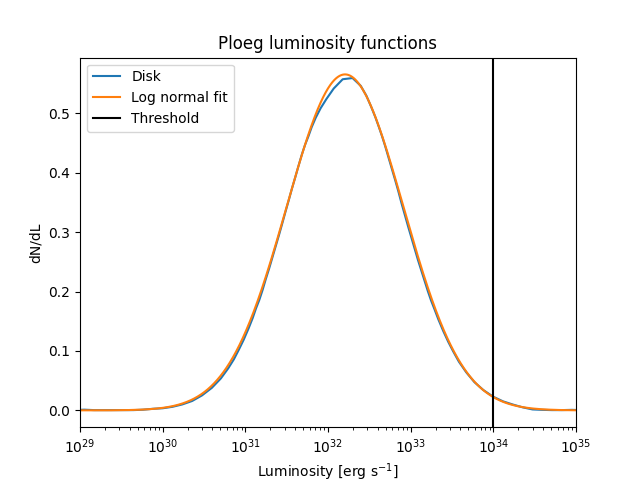
\includegraphics[width=0.5\textwidth]{get-estimates.png}
    \caption{Luminosity function to be integrated over. The blue plot is the extracted function, while the orange is a log-normal fit to it. The black line is the threshold luminosity $L_{th}$, sometimes used as an integration bound.}
    \label{fig:func}
\end{figure}



\section{Methods}
Methods employed for both integrals approximate the luminosity function as piecewise-linear, that is:
\begin{equation}
\frac{dN}{dL}(x) \approx \begin{cases}
    \frac{y_2 - y_1}{x_2 - x_1}(x - x_1) + y_1 & x_1 \leq x < x_2 \\
    \frac{y_3 - y_2}{x_3 - x_2}(x - x_2) + y_2 & x_2 \leq x < x_3 \\
    \vdots & \vdots \\
    \frac{y_N - y_{N-1}}{x_N - x_{N-1}}(x - x_{N-1}) + y_{N-1} & x_{N-1} \leq x \leq x_{N} \\
    \label{eqn:approx}
\end{cases}
\end{equation}
where $x_1,\dots, x_N$ and $y_1,\dots, y_N$ are the points extracted from the luminosity function found in the literature, structured so that $x_1 < x_2 < \dots < x_N$ and $y_i = \frac{dN}{dL}(x_i)$.

The bounds of the integral are then restricted to the domain $[x_1, x_N]$. For example, the integral over $[0, \infty)$ becomes an integral over $[x_1, x_N]$.

\subsection{Number integral}
We will compute the first integral given in equation \ref{eqn:ints} by integrating the components of equation \ref{eqn:approx}. The result is
\begin{equation*}
    \int_{L_{min}}^\infty \frac{dN}{dL}dL = \int_{L_{min}}^{x_{n}}\frac{y_{min} - y_n}{L_{min} - x_n}\parens{x - L_{min}} + y_{n-1} dx + \sum_{i = n}^{N-1}\int_{x_i}^{x_{i+1}}\frac{y_{i+1} - y_i}{x_{i+1} - x_i}\parens{x - x_i} + y_i dx
\end{equation*}
where we have chosen $n$ such that $x_{n-1} \leq L_{min} < x_n$, and set $y_{min} = \frac{y_{n} - y_{n-1}}{x_{n} - x_{n-1}}\parens{L_{min} - x_{n-1}} + y_{n-1}$. Performing the integral, we get
\begin{equation}
    \int_{L_{min}}^\infty \frac{dN}{dL}dL = \frac{1}{2} \parens{x_n - L_{min}}\parens{y_n + y_{min}} + \sum_{i=n}^{N-1}\frac{1}{2} \parens{x_{i+1} - x_i}\parens{y_{i+1} + y_{i}}
\end{equation}
which is equivalent to trapezoidal integration. This series can be simplified, but we will not do so.


\subsection{Luminosity integral}
The same process can be applied to integrate the second integral given in equation \ref{eqn:ints}. We will compute
\begin{equation*}
    \int_{L_{min}}^\infty \frac{dN}{dL}dL = \int_{L_{min}}^{x_{n}}\frac{y_{min} - y_n}{L_{min} - x_n}\parens{x^2 - xL_{min}} + xy_{n-1} dx + \sum_{i = n}^{N-1}\int_{x_i}^{x_{i+1}}\frac{y_{i+1} - y_i}{x_{i+1} - x_i}\parens{x^2 - xx_i} + xy_i dx.
\end{equation*}
The result is
\begin{align}\begin{split}
    \int_{L_{min}}^\infty \frac{dN}{dL}dL & = \frac{1}{6}\parens{x_n - L_{min}}\brackets{y_{min}\parens{2 L_{min} + x_n} + y_n\parens{L_{min} + 2x_n}}\\ 
    &+ \frac{1}{6}\sum_{i=n}^{N-1}\parens{x_{i+1} - x_{i}}\brackets{y_{i}\parens{2 x_{i} + x_{i+1}} + y_{i+1}\parens{x_{i} + 2x_{i+1}}}.
\end{split}\end{align}


\section{Results}
We may compare the accuracy of this numerical method by fitting a log-normal distribution to the luminosity function and comparing the analytical and numerical results of the integrals in equation \ref{eqn:ints}. The log normal distribution used is 
\begin{equation}
    \frac{dN}{dL} = \frac{\log_{10} e}{\sigma \sqrt{2\pi} L}\expp{-\frac{\parens{\log_{10} L - \log_{10} L_0}^2}{2\sigma^2}},
    \label{eqn:log-normal}
\end{equation}
and the fit achieved values of $L_0 = \SI{1.6084e+32}{\erg\per\second}$ and $\sigma=0.7003$. The integrals were computed analytically, and the function was sampled with $N$ points in $[\SI{e29}{\erg\per\second}, \SI{e35}{\erg\per\second}]$ spaced evenly in log space. The percent deviation of the numerical integrals from the analytical integrals is shown in figure \ref{fig:compare-integral}. The percent deviations as calculated for four points commonly used in the jan-2021 summary of this UROP are shown in table \ref{tab:calc-points}.


\begin{figure}[h]
    \centering
    \begin{subfigure}{.49\textwidth}
        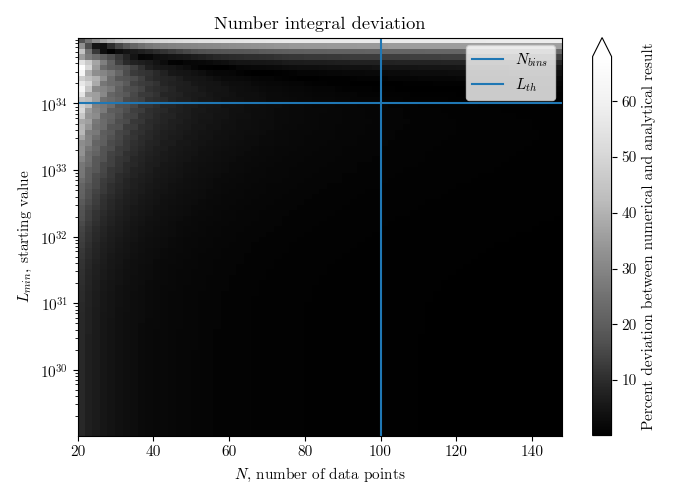
\includegraphics[width=0.99\linewidth]{num-integral-deviation.png}
        \caption{Number integral}
    \end{subfigure}
    \begin{subfigure}{.49\textwidth}
        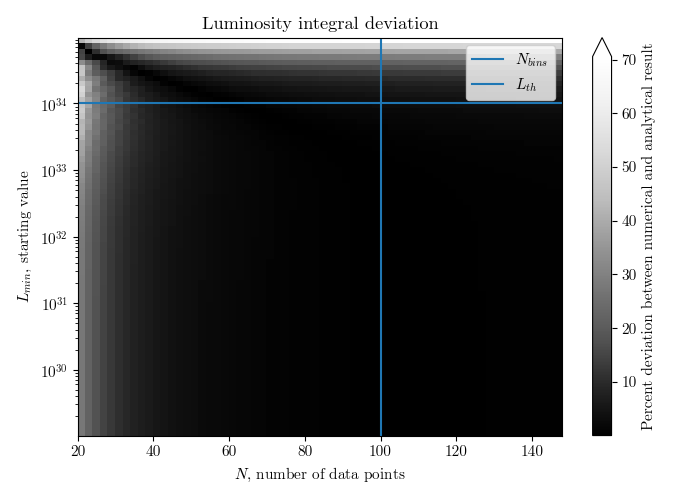
\includegraphics[width=0.99\linewidth]{lum-integral-deviation.png}
        \caption{Luminosity integral}
    \end{subfigure}
    \caption{Percent deviation between the numerical integral, calculated by sampling $N$ points, equally-spaced in log space, from a log normal distribution and using the described methods to integrate over the range from $L_{min}$ to the edge of the domain, which was $\SI{e35}{\erg\per\second}$ here.}
    \label{fig:compare-integral}
\end{figure}


\begin{table}[h]
    \centering
    \begin{tabular}{|c|c|c|}
        \hline
        & Number integral & Luminosity integral \\ \hline
        $L_{min} = \SI{e29}{\erg\per\second}$ & 0.321\% & 0.0796\%\\ \hline
        $L_{min} = L_{th} = \SI{e34}{\erg\per\second}$ & 0.934\% & 3.65\% \\ \hline
    \end{tabular}
    \caption{Percent deviations between the numerical and analytical values of the integrals shown in equation \ref{eqn:ints}, for the log-normal fit to Ploeg et al.'s data.}
    \label{tab:calc-points}
\end{table}


\section{Conclusion}
We developed a method to numerically integrate a luminosity function and its expectation value, and affirmed that it was accurate to within four percent at relevant points.

The position-dependent sensitivity model cited in the jan-2021 summary may be more inaccurate than table \ref{tab:calc-points} suggests, because for pixels near the galactic plane, the threshold luminosity can rise to as much as five times the value of $L_{th}$ used here.

The luminosity function extracted from Ploeg et al. does not match the log-normal fit perfectly, particularly at high luminosities. The deviations present between the ``custom'' luminosity function and the log normal fit in the jan-2021 summary are most likely caused by this disagreement, not numerical error.


\begin{thebibliography}{99}
    \bibitem{ploeg} H. Ploeg, C. Gordon, R. Crocker, O. Macias. ``Comparing the Galactic Bulge and Galactic Disk Millisecond Pulsars.'' arXiv:2008.10821v2 (2020).

\end{thebibliography}


\end{document}